%!TEX root = ../../dissertation.tex
%%%%%%%%%%%%%%%%%%%%%%%%%%%%%%%%%%%%%%%%%%%%%%%%%%%%%%%%%%%%%%%%%%%%%%%%%%%%%%%%
\section{Mobile Reliable Streaming Simulations}
\label{c6:sec:mobilestreamingtestbed}

However, some experiments can not be easily conducted in active measurement testbeds, for example due to the necessary scale to achieve meaningful results. Especially, new protocols or adaptations to existing ones are preferentially first tested in a network simulation. Simulation frameworks are especially important for mobile networks, as acquiring packet-level traces and information about every node in an actual commercially operating cellular network is nigh impossible due to the users' privacy and the provider's business concerns.

While there are some active measurement studies specifically targeted at reliable streaming in mobile networks, e.g., \cite{Muller:2012:EDA:2151677.2151686}, most are conducted either in fixed networks or using simulation frameworks. Therefore, to better evaluate reliable streaming, it would be very desirable to find an existing framework, that covers all important aspect in 3G or 4G mobile networks.

There are a number of network simulators readily available for use, both commercial as well as \gls{FOSS}. But only a small subset of them has the capability (or can be extended) to simulate \gls{3G} or LTE networks. Even further, most radio network capable simulators only concern themselves with the physical radio link and completely neglect all other network paths, especially the core and all control plane signaling interactions. 

The following list overviews current publicly available simulation frameworks with \gls{3G}/\gls{LTE} support:

\begin{itemize}
	\item An external \gls{UMTS} module\footnote{\url{http://net.infocom.uniroma1.it/reti_files/reti_downloads.htm}} is available for the no longer maintained \textbf{ns-2} simulation framework. A further separate collection of patches\footnote{\url{http://seacorn.cs.ucy.ac.cy/eumtssim/}} also extends ns-2 with \gls{UMTS} radio link capabilities~\cite{vranjevs2011use} but it is not publicly available.

	Both are as of August 2014 no longer being developed and not up-to-date to the newest specifications. They also focus solely on the user plane radio physical and link layer of \gls{UMTS}.

	\item Another third-party radio link layer simulation model is available for \textbf{MATLAB}\footnote{\url{http://www.nt.tuwien.ac.at/research/mobile-communications/lte-simulators/}}~\cite{mehlfuhrer2011vienna}.

	\item A standalone \gls{LTE} simulation\footnote{\url{http://telematics.poliba.it/index.php/en/lte-sim}}~\cite{5634134} includes models for some \gls{LTE} nodes, including the \gls{eNB} and \gls{MME} and implements a selection of protocols (\gls{PDCP}, \gls{RLC}, and \gls{RRC}).

	However, the implementation of these nodes and protocols is rudimentary at best and is not even close to the actual specification. Additionally, the simulator lacks a \gls{TCP}/\gls{IP} stack as \gls{IP} is reduced to its basic functionality and \gls{TCP} is completely absent.

	\item A framework dubbed SimuLTE\footnote{\url{https://github.com/inet-framework/simulte}} is available for \textbf{Omnet++}\footnote{\url{http://www.omnetpp.org/}}. Included are the user plane aspects of the radio link and some basic \gls{SGW} and \gls{PGW} functionality.

	\item The \textbf{ns-3}\footnote{\url{http://www.nsnam.org}} simulator already contains an \gls{LTE}/\gls{EPC} module called LENA\footnote{\url{http://networks.cttc.es/mobile-networks/software-tools/lena/}}~\cite{Baldo:2013:OSM:2507924.2507940} with features similar to SimuLTE. Again, only user plane \gls{SGW}/\gls{PGW} functionality is present with an initial \gls{GTP-U} implementation.
\end{itemize}

The goal here is to simulate reliable streaming in a realistic mobile environment. That includes both a complete horizontal network path --- both the radio link as well as the core network --- as well as a vertical network stack --- comprising both user plane and control plane.

Unfortunately, none of the above feature a complete representation, which can be at least partially attributed to the complexity of the \gls{3GPP} specifications. Nonetheless, the simulators could still provide a viable basis for a mobile streaming framework while keeping the limitations in mind.Between these a decision needs to be made as to the basis of the mobile streaming simulation framework. 

Ultimately, the choice fell on ns-3 with the LENA module. Alongside with SimuLTE it has the most complete \gls{LTE} representation. And targeting \gls{LTE} networks seems to be the more future-proof path in the the long term. With the exception of Omnet++, which has comparable capabilities, ns-3's \gls{TCP}/\gls{IP} is much more complete and realistic than that of the other frameworks. Additionally, it can also incorporate the actual \gls{TCP}/\gls{IP} of older Linux kernels with NSC\footnote{\url{http://research.wand.net.nz/software/nsc.php}}. As an additional feature, ns-3 can also act as a network emulator for real network traffic. This will be exploited in the upcoming model.

In the long run, to better represent actual mobile networks the base radio framework in ns-3 would need to be extended with more control plane aspects and adapted to 


%%%%%%%%%%%%%%%%%%%%%%%%%%%%%%%%%%%%%%%%%%%%%%%%%%%%%%%%%%%%%%%%%%%%%%%%%%%%%%%%
\subsection{Simulating Mobile Reliable Streaming in ns-3}

With ns-3 chosen and the core network model set, the task is now to define and simulate reliable streaming on top of the \gls{LTE} network.



%%

\subsubsection{Simulated Streaming Model}
Reliable streaming type implemented:

According to the classification and playback modeling from Sections~\ref{c3:sec:background} and \ref{c3:sec:model} the simulated model is a pull-based segmented video streaming system using \gls{TCP}.

Model 1:

4 threshold segmented streaming
	Playback stop if below threshold 1 default \SI{0.5}{\second}
	Transmission start if below threshold 2 (request new segments), default \SI{2.5}{\second}
	Playback start if above threshold 3, default \SI{5}{\second}
	Transmission stop if above threshold 4 (request no new segments)


directly on top of TCP
pull-based with request per segment; could also use HTTP here, but should not make much difference, only slightly more overhead through http header


Model 2:

planned not fully implemented 
6 threshold adaptive reliable streaming


%% ! <-- !
%%


%%
\subsubsection{Simulation and Emulation Setups}
Different Approaches

\begin{figure}[htb]
\centering
\includegraphics[width=0.6\textwidth]{images/streaming-simulation.pdf}
\caption{\gls{LTE} reliable streaming simulation testebd.}
\label{c5:fig:streaming-simulation}
\end{figure}


Implement a Reliable Streaming Traffic Generator ns-3 Application and a streaming receiver client application.

Describe Streaming Simulation Model and Variables

Describe ns-3/LENA implementation

 Use LENA to transport streams


%% emu

Use introduced streaming evaluation approaches in a mobile network environment

But do not want to use real network, as conditions are hard to manage and reproduce.

comparable to the initial (simple) network emulation used in the measurement framework in Section~\ref{c3:sec:measurements} using static values
here it acts as a dynamic network emulator, delaying packets based on its pass-through time through the network, while also adding packet loss.

Therefore, use an emulated network provided by the ns-3 network simulator. But transmit real traffic through it, i.e., use it as an emulator and bridges. \ref{c5:fig:streaming-simulation} \ref{c5:fig:streaming-hybrid}


\begin{figure}[htb]
\centering
\includegraphics[width=\textwidth]{images/streaming-hybrid.pdf}
\caption{Future testbed iteration: hybrid of ns-3 LTE simulation and actual or emulated streaming client and server bridged to it.}
\label{c5:fig:streaming-hybrid}
\end{figure}



%%
\subsubsection{Scenario Evaluation}
Evaluated Scenarios (and scenarios that are worthy of evaluation in the fture)

 test case 1: adaptability of diverse reliable video streaming to LTE and mobile networks, by altering latency, loss, bandwidth

 test case 2a (future): influence of mobility effects on reliable streaming
 test case 2b (future): effect of cross-layer information in mobility case





\begin{figure}[htb]
\centering
\includegraphics[width=1.0\textwidth]{images/R-ltesim-plotbuffer-time.pdf}
\caption{R-ltesim-plotbuffer-time.pdf}
\label{c5:fig:ltesim-plotbuffer-time}
\end{figure}


\begin{figure}[htb]
\centering
\includegraphics[width=1.0\textwidth]{images/R-ltesim-bwseries-numstalls.pdf}
\caption{R-ltesim-bwseries-numstalls.pdf}
\label{c5:fig:ltesim-bwseries-numstalls}
\end{figure}

\begin{figure}[htb]
\centering
\includegraphics[width=1.0\textwidth]{images/R-ltesim-bwseries-stallduration.pdf}
\caption{R-ltesim-bwseries-stallduration.pdf}
\label{c5:fig:ltesim-bwseries-stallduration}
\end{figure}

\begin{figure}[htb]
\centering
\includegraphics[width=1.0\textwidth]{images/R-ltesim-latencyseries-numstalls.pdf}
\caption{R-ltesim-latencyseries-numstalls.pdf}
\label{c5:fig:ltesim-latencyseries-numstalls}
\end{figure}

\begin{figure}[htb]
\centering
\includegraphics[width=1.0\textwidth]{images/R-ltesim-latencyseries-stallduration.pdf}
\caption{R-ltesim-latencyseries-stallduration.pdf}
\label{c5:fig:ltesim-latencyseries-stallduration}
\end{figure}








% \begin{figure}[htb]
% \centering
% \includegraphics[width=\textwidth]{images/lte-testbed.pdf}
% \caption{\gls{LTE} Streaming Evaluation Setup and Action Plan}
% \label{fig:lte-testbed}
% \end{figure}



% \url{http://www.valid8.com/UMTS_Core_Network_Simulator.html} Not publicly available and commercial
% also seems to focus on the circuit switched domain


% Only commercial: UMTS model in OPNET (which was renamed to Riverbed Modeler)\footnote{\url{http://www.riverbed.com/products/performance-management-control/network-performance-management/network-simulation.html}} 
% again radio and user plane focused

%\url{http://www.nsnam.org/docs/release/3.20/doxygen/group__lte.html}
%\url{http://www.nsnam.org/docs/release/3.20/models/html/lte.html}

%Reasoning why ns-3/LENA will be used here.
%but combined with ns-3 offers almost complete representation of a vanilla network and transport level network stack
